%!TEX root = ./ERL Industrial Robots.tex

%--------------------------------------------------------------------
%--------------------------------------------------------------------
\subsection{Navigation Functionality (Shared with RoboCup@Work)}
\label{ssec:Navigation}

%--------------------------------------------------------------------
% IST-ID
\subsubsection{Functionality Description}
\label{sssec:FooOMDescription}

This benchmark evaluates the robot navigation capability.

%--------------------------------------------------------------------
% IST-ID
\subsubsection{Feature Variation}
\label{sssec:FooOMVariation}

This benchmark has the following feature variation:
\begin{itemize}
  \item{Distinct starting points, waypoints, and goal positions.}
  \item{Different number of waypoints to reach the goal.}
  \item{Different number of obstacles blocking the path.}
\end{itemize}

%--------------------------------------------------------------------
% IST-ID
\subsubsection{Input Provided}
\label{sssec:FooOMInput}

The robot will receive the following information:
\begin{itemize}
  \item{The starting position.}
  \item{The number of waypoints that the robot must visit.}
  \item{The coordinates of the waypoints that the robot must visit (the last waypoint corresponds to the goal position). A waypoint encapsulates a X, Y and $\theta$. The coordinates are given in the testbed reference frame (which will be defined on site and provided during the first day to the teams).}
  %\item{The maximum time allowed for the robot to go from each waypoint to the next waypoint, without penalization.} 
  \item{The deadline for the robot to go from each waypoint to the next, receiving points for that path. If robots spent more time than this deadline when going from one waypoint to the next waypoint, they will not get points on that path.}% More information will be provided at least eight weeks before the competition in the \ro Wiki~\cite{rockin:wiki:2015}}.
\end{itemize}

%--------------------------------------------------------------------
% IST-ID
\subsubsection{Expected Robot Behavior or Output}
\label{sssec:FooOMOutput}

Teams are required to set their robot on a specific starting position (that will be given to the teams before each run). Then, the robot receives, through the CFH, the start signal, as well as an ordered list of waypoints that it must reach. The robot must follow the order in which the waypoints are sent from the testbed, sending back a signal to the CFH, each time it reaches a waypoint. The evaluation of the navigation will take into account the following three items (a complete formula for the scoring will be presented at Sec.~\ref{sssec:FooOMScoring}):
\begin{itemize}
  \item The distance between the robot's position and the respective position of the waypoint. It will be accounted both the Euclidean distance between the waypoint and the robot, and the difference in the orientation.
  \item The time spent by the robot to go from each waypoint to the next waypoint. 
  \item The number of times that the robot hits each obstacle. If the robot hits the same obstacle more than once, it will count as multiple hits.
\end{itemize}

The functionality benchmark ends as soon as one of the following situations occurs:
\begin{itemize}
  \item The robot reaches the last waypoint which corresponds to the goal position. 
  \item The time available for the functionality benchmark expires.
  \item The robot damages any of the obstacles.
  \item The robot pushes or continually touches an obstacle for more than 3 seconds.
  \item The robot forces its path through an obstacle.
\end{itemize}

%--------------------------------------------------------------------
% IST-ID
\subsubsection{Procedures and Rules}
\label{sssec:FooOMProcedures}
All teams are required to perform this functionality benchmark according to the steps mentioned below. The task must be performed exclusively in autonomous mode. No teleoperation is allowed. Teams will have up to ten minutes to complete the functionality benchmark. Two minutes to move the robot to the correct starting position plus eight minutes to do the benchmarking.

\begin{description}
  \item [Step 1] The team is required to start their robot on a pre-defined starting position. This starting position will be given to the teams before each run.
  \item [Step 2] When the procedure starts, the robot receives a sequence of waypoints that it must follow in the respective order, sending back a signal through the CFH, each time it reaches a waypoint. The robot must avoid hitting any obstacle it encounters in its path.
  \item [Step 3] The procedure stops when the robot notifies it has reached the goal position (which corresponds to the last waypoint), when the time given to complete the test expires, or when the robot hard-hits an obstacle.
\end{description}


%The obstacles can be of three types: 
%\begin{itemize}
%  \item \textbf{Static and previously mapped}: Hardware already present in the house such as furniture, doors, walls, defined in \ref{sssec:NRObjects}. The teams should already have this obstacles mapped from set-up days. These items will not change during this functionality benchmark.
%  \item \textbf{Static}: Items Granny Annie left lying on the ground. The obstacles may be of different shapes and sizes, are not previously known by the teams, and may be different in between runs.
%  \item \textbf{Dynamic}: Granny Annie's visitors. People moving inside the house. Obviously, the movement people will do is unpredictable.
%\end{itemize}



%--------------------------------------------------------------------
% POLIMI
\subsubsection{Acquisition of Benchmarking Data}
\label{sssec:FooOMData}
During the execution of the benchmark, the internal data described in the following table will be collected

\begin{table}[h]
\centering
\begin{footnotesize}
\begin{tabular}{|l|l|l|l|}
\hline
Topic	&	Type		&	Frame Id		&	Notes \\ \hline\hline
/rockin/robot\_pose\_waypoint\tablefootnote{The 2D robot pose, once each waypoint is reached, at the floor level, i.e., $z=0$ and only yaw rotation.} & geometry\_msgs/PoseStamped & /map & when reached \\ \hline
/rockin/marker\_pose\_waypoint\tablefootnote{The 3D pose of the marker in 6 degrees of freedom once each waypoint is reached.} & geometry\_msgs\/PoseStamped	& /map & when reached \\ \hline
\end{tabular}
\end{footnotesize}
\end{table}

This functionality benchmark will be fully automated (no human operation will be allowed) and, for that, the robot has to communicate with the CFH. It will receive the list of target waypoints from the CFH and it must send back a signal, each time it reaches a waypoint.
\begin{table}[h]
\centering
\begin{footnotesize}
\begin{tabular}{|l|l|p{5cm}|}
\hline
 Topic	&	Type  	  &	Notes \\ \hline\hline
 /roaw\_cfh/goal & geometry\_msgs/Pose2D & List of waypoints, sent by the CFH to the robot, when starting the task. \\ \hline
 /roaw\_cfh/reached\_waypoint & roaw\_cfh\_comm\_ros/UInt8 & Message sent by the robot to the CFH, when reaching a point. It must include the number of the respective waypoint in the sequence (starting from zero). \\ \hline
\end{tabular}
\end{footnotesize}
\end{table}


%--------------------------------------------------------------------
% IST-ID + ROME + POLIMI
\subsubsection{Scoring and Ranking}
\label{sssec:FooOMScoring}

\begin{figure}[t!]
  \centering
  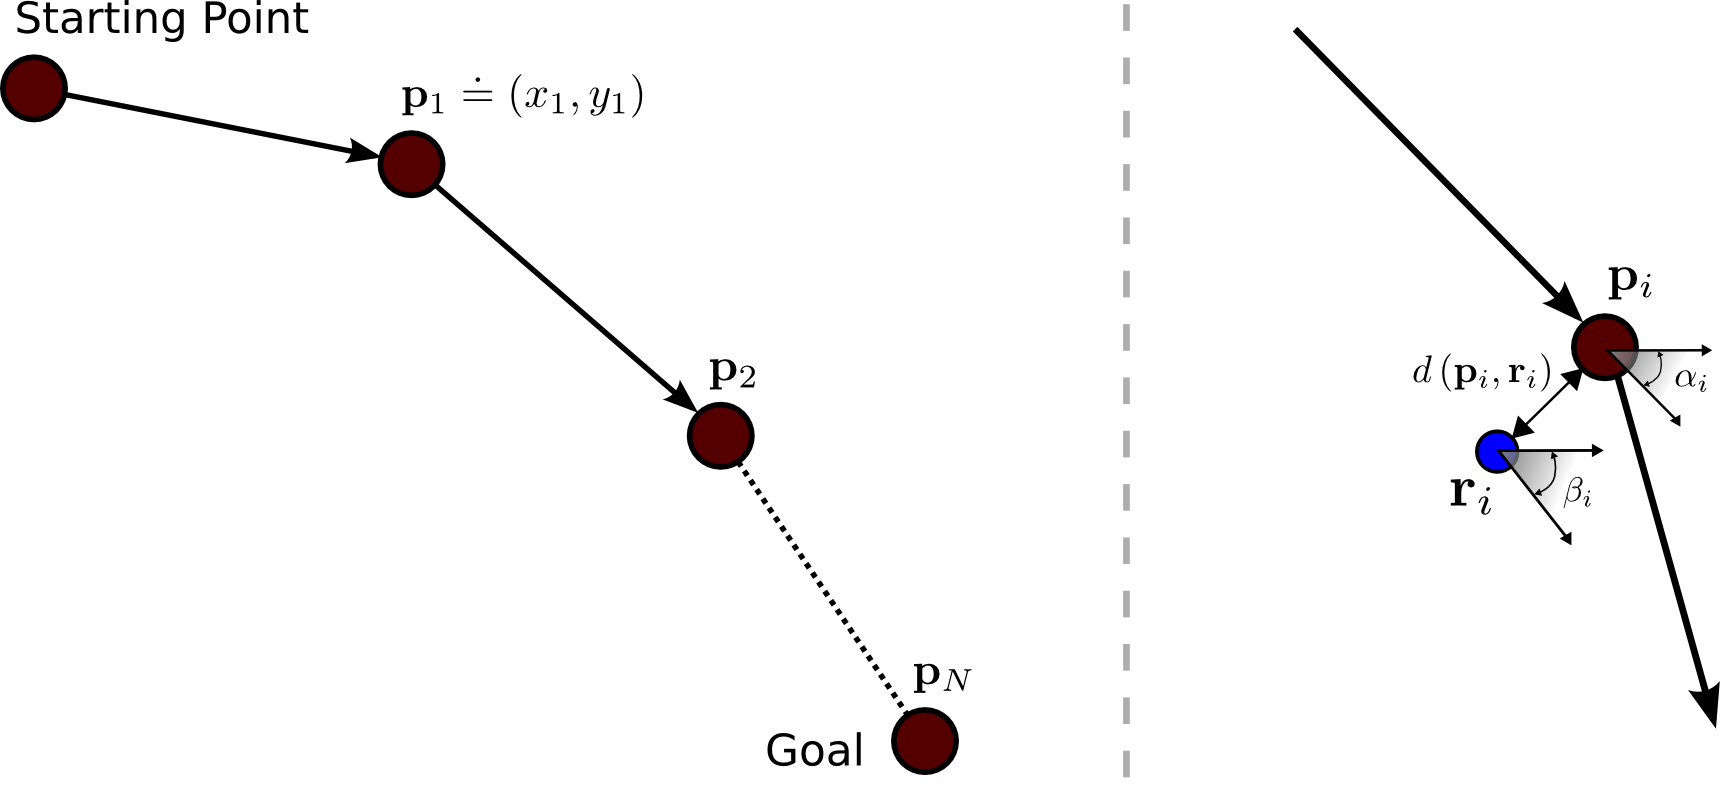
\includegraphics[width=0.8\textwidth]{./fig/FBM/athome/fbm2_navigation/drawing_final.png}
  \caption{Depiction of the sequence of waypoints that the robot must follow, during the navigation functionality benchmark.} \label{fig:navigation_waypoints}
\end{figure}
 
At each run and for each team, three metrics will be used to score the performance: Accuracy, number of obstacle hits, execution time. 

\begin{itemize}
  \item{Accuracy scoring will be based on the mathematical means of the distance from the waypoints and the corresponding orientation error. The distance mean from the robot to the target waypoint follows the equation
\begin{equation}
    A = \frac{1}{N}\sum_{i}^{N}d\left(\mathbf{p}_i, \mathbf{r}_i\right),
    \nonumber
\end{equation}
where $d\left(\mathbf{p}_i, \mathbf{r}_i\right)$ is the Euclidean distance from the robot's position $ \mathbf{r}_i$ to the target waypoint $\mathbf{p}_i$ (as shown in Figure \ref{fig:navigation_waypoints}) and $N$ the total number of points. 

Considering the orientation, the mean is 
\begin{equation}
    B = \frac{1}{N}\sum_{i}^{N}\delta\left(\alpha_i, \beta _i\right),
    \nonumber
\end{equation}

where $\delta\left(\alpha, \beta \right)$ is the absolute value of the difference between the desired waypoint orientation $\mathbf{\alpha}$ and the robot's orientation $\beta$, such that $\delta\left(\alpha, \beta \right)=\left | \alpha- \beta \right |$ 


After the computation of these accuracy scorings, they will be discretized and fitted in one of the following groups:
\begin{itemize}
    \item 1: $A<10cm$ AND $B<20^{\circ}$;
    \item 2: $A<30cm$ AND $B<45^{\circ}$;
    \item 3: $A<50cm$ AND $B<90^{\circ}$;
    \item 4: $A<80cm$ AND $B>90^{\circ}$;
\end{itemize}
A lower group number corresponds to the better performance. Therefore, teams will be ranked starting from group 1. Note that for a team to be placed in any of the groups, it \textbf{must} respect the limits for $A$ and $B$. If a team has a score that does not fit any of groups defined above (e.g. mean of the error above 80cm), it will not receive scoring in the respective Functionality Benchmark run;}
  \item{If more than one team is found inside each of the previously defined group, the number of obstacle hits will be used as a tie breaker, where the team with less hits will be ranked first and so on. Note that hits will only be considered as a tie breaker, $i.e.$, a team in group 2 will never be ranked first than any team in 1, despite of the number of hits (note that a class of hard hits was defined which, if they happen, the procedure stops);}
  \item{If teams are still tied, time will be the decisive tie breaker.}
  \end{itemize}

Note that throughout the competition and according to the teams performance, the thresholds for the classes of $A$ and $B$ can be changed.

%--------------------------------------------------------------------
% EOF
%--------------------------------------------------------------------
